\section{Metodologia}\label{sec:methodology}

O protocolo separa a representação das propriedades, a resposta de uma geometria fixa e o redimensionamento. O experimento principal substitui somente a rigidez: as demais propriedades, ações, limites e hipóteses são comuns aos dois cenários de cada par espécie--vão. Esse controle permite atribuir a diferença observada à representação da rigidez dentro do modelo adotado. Uma comparação de conjuntos completos de propriedades constituirá uma extensão condicionada à definição e à justificativa dos dados complementares.

\subsection{Sistema estrutural e modelo paramétrico}\label{sec:system}

O sistema considerado é uma superestrutura de vão único simplesmente apoiado, com peças retangulares de tabuleiro apoiadas sobre longarinas circulares de madeira roliça, distribuídas ao longo da largura da pista. As ações incluem peso próprio, carga permanente adicional, cargas de roda e carga distribuída de multidão. A transferência das ações e a obtenção de esforços e deslocamentos são realizadas pelo modelo analítico paramétrico da plataforma ReliaBridge \parencite{ReliaBridge2026}.

\begin{figure}[!ht]
\centering
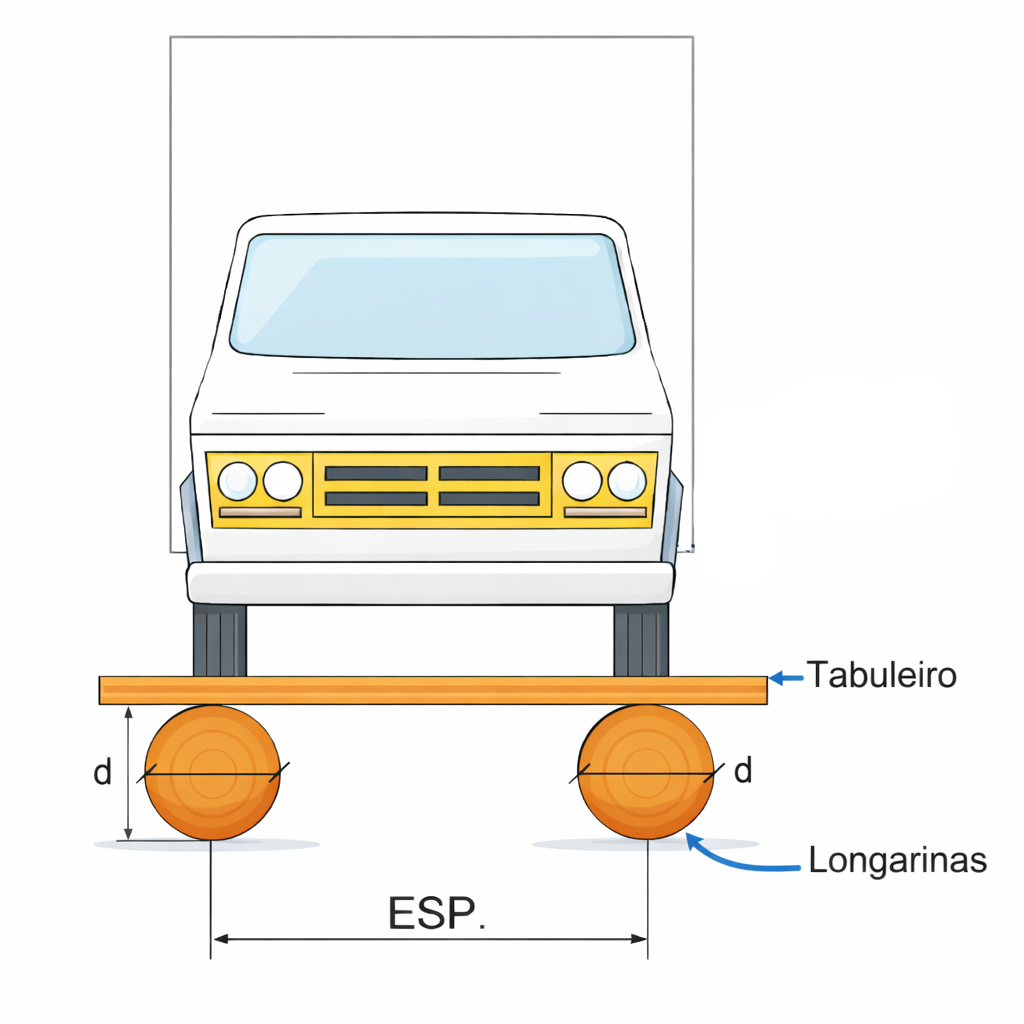
\includegraphics[width=0.5\textwidth]{figuras/caminhao.png}
\caption{Representação conceitual da superestrutura considerada.}
\label{fig:system}
\end{figure}

A análise de propriedades obtidas em ensaios de caracterização não constitui validação experimental de peças roliças de dimensão estrutural. A aplicação à ponte é uma investigação numérica condicionada ao modelo e às hipóteses de transferência dessas propriedades.

\subsection{Hipóteses e verificações de projeto}\label{sec:verificacao}

Para cada comparação serão documentados geometria, ações, combinações, resistência à flexão, resistência ao cisalhamento, densidade, relação entre módulos e parâmetros de fluência. Cada entrada será identificada como experimental, estimada ou adotada. As verificações compreendem flexão e cisalhamento das longarinas, deslocamentos, flexão do tabuleiro e limites geométricos. Os critérios de serviço incluem a flecha final quase permanente e a flecha variável, conforme a Seção~\ref{sec:restricoes}.

\subsection{Geometria, discretização e volume}\label{sec:geometria}

A formulação de dimensionamento reaproveita o núcleo mecânico do manuscrito da plataforma, baseado no roteiro de pontes de madeira de \textcite{CALIL2006}, e explicita as hipóteses necessárias à comparação entre materiais. As longarinas são representadas por vigas prismáticas circulares; as pranchas do tabuleiro vencem transversalmente os vãos entre longarinas. Com $B$ denotando a largura da pista, as propriedades das seções são
\begin{equation}
 A_\ell=\frac{\pi d^2}{4},\quad I_\ell=\frac{\pi d^4}{64},\quad
 W_\ell=\frac{\pi d^3}{32},\qquad
 A_t=b_wh,\quad I_t=\frac{b_wh^3}{12},\quad W_t=\frac{b_wh^2}{6}.
\label{eq:secoes}
\end{equation}
O diâmetro $d$ é o diâmetro uniforme de cálculo. A representação de uma tora afilada por um diâmetro equivalente deverá ser compatibilizada com o critério normativo aplicável; o volume de uma peça prismática equivalente não é necessariamente o volume comercial da tora afilada.

A disposição construtiva considera números inteiros de peças. Para um comprimento disponível $D$, largura de peça $w$ e espaçamento livre proposto $s$, a rotina geométrica examina os inteiros adjacentes a $(D+s)/(w+s)$ e calcula
\begin{equation}
 s_{corr}=\frac{D-nw}{n-1},\qquad n\geq2.
\label{eq:acomodacao}
\end{equation}
Empregam-se $(D,w)=(B,d)$ para as longarinas e $(D,w)=(L,b_w)$ para as pranchas. Entre as alternativas, priorizam-se a viabilidade dos espaçamentos e a proximidade ao valor proposto. Essa operação introduz descontinuidades no espaço de projeto e permite que o número de peças varie durante a busca. O problema, portanto, não é uma simples otimização contínua de seções com número de elementos fixo.

O volume de madeira contabilizado é
\begin{equation}
 V(\mathbf{x})=n_\ell A_\ell L+n_t A_t B.
\label{eq:volume_modelo}
\end{equation}
Esse indicador cobre longarinas e pranchas, sem representar diretamente custo, carbono incorporado, perdas de corte ou volume de fundações e ligações.

\subsection{Ações e distribuição transversal}\label{sec:acoes}

A configuração de referência transportada do manuscrito da Matéria utiliza o veículo TB-240 associado à \textcite{nbr7188}: seis rodas de $P=40$~kN, em três eixos espaçados de $a=1{,}5$~m, correspondendo a 80~kN por eixo e 240~kN por veículo. A carga de multidão de referência é $q_A=4$~kN/m\textsuperscript{2}. A aplicação dessa configuração à via estudada e as combinações correspondentes deverão ser documentadas na definição final dos casos.

Para peso específico $\gamma_{mat}=9{,}81\rho_{ap}/1000$ em kN/m\textsuperscript{3}, o peso próprio médio do tabuleiro por unidade de área é $g_{A,t}=\gamma_{mat,t}n_tA_t/L$. Definindo $b_{tr,i}$ como largura tributária da longarina $i$ e $g_{A,ad}$ como carga permanente adicional, tem-se
\begin{equation}
 g_{\ell,i}=\gamma_{mat,\ell}A_\ell+(g_{A,t}+g_{A,ad})b_{tr,i},
 \qquad q_{\ell,i}=q_A b_{tr,i}.
\label{eq:acoes_lineares}
\end{equation}
A largura tributária tem dimensão de comprimento e deve ser definida a partir da distribuição efetiva das cargas e das posições dos apoios. O espaçamento livre $s_{corr}$, a distância entre eixos das longarinas $s_{corr}+d$ e o vão de cálculo do tabuleiro $\ell_t$ são grandezas distintas. Para cargas concentradas, a parcela recebida pela longarina depende também da posição transversal da roda; a adoção de uma roda inteira sobre uma longarina constitui uma hipótese de carregamento a justificar, e não uma consequência da conversão de carga de área em carga linear.

\begin{fillblock}
\noindent\textbf{[COMPATIBILIZAÇÃO IDENTIFICADA NA TRANSFERÊNCIA]} A implementação atual utiliza o espaçamento livre corrigido como largura tributária e como vão do tabuleiro. Antes das novas rodadas, conferir a representação dos apoios, as longarinas de borda e o balanço de cargas, exigindo que a distribuição preserve a carga total. A formulação acima distingue essas grandezas; sua adoção definitiva requer compatibilização com o código. Esta revisão do manuscrito não altera o programa de cálculo.
\end{fillblock}

\subsection{Esforços e resposta elástica}\label{sec:esforcos}

Adotam-se pequenas deformações e comportamento elástico linear de vigas de Euler--Bernoulli, sem deformação por cisalhamento. Para carga permanente uniforme $g_\ell$, as expressões são
\begin{equation}
 M_{G,k}=\frac{g_\ell L^2}{8},\qquad
 Q_{G,k}=\frac{g_\ell L}{2},\qquad
 \delta_{G,k}=\frac{5g_\ell L^4}{384E_{M0}I_\ell}.
\label{eq:permanentes_modelo}
\end{equation}
No cálculo em kN e m, os módulos e resistências são convertidos de MPa para kN/m\textsuperscript{2}, multiplicando-se por $10^3$.

Para a posição simétrica de três cargas iguais, com uma carga no meio do vão e as demais afastadas de $a$, o momento e o deslocamento no meio do vão são
\begin{align}
 M_{P,k}(L/2)&=\frac{3PL}{4}-Pa,\label{eq:momento_tres_rodas}\\
 \delta_{P,k}(L/2)&=\frac{P}{48E_{M0}I_\ell}
 \left[L^3+2b(3L^2-4b^2)\right],\qquad b=\frac{L-2a}{2}.
\label{eq:flecha_tres_rodas}
\end{align}
Essas expressões pressupõem que as três cargas estejam sobre o vão, com $L\geq2a$; $a$ é o espaçamento entre eixos do veículo. São soluções de uma configuração especificada e não substituem, sem verificação, a envoltória de todas as posições possíveis do veículo.

A conferência independente da carga móvel será feita por linhas de influência. Para uma seção $x$ e uma carga na posição $z$, a linha de influência do momento da viga biapoiada é
\begin{equation}
 \eta_M(x,z)=
 \begin{cases}
 z(L-x)/L,&0\leq z\leq x,\\
 x(L-z)/L,&x<z\leq L.
 \end{cases}
\label{eq:linha_influencia}
\end{equation}
Para cada posição $\zeta$ do veículo, somam-se as rodas que efetivamente estão sobre o vão e integra-se a carga distribuída sobre a região carregada $\Omega(\zeta)$:
\begin{equation}
 M_Q(x;\zeta)=\sum_{j:z_j(\zeta)\in[0,L]}P_j\eta_M(x,z_j)
 +\int_{\Omega(\zeta)}q_\ell(z)\eta_M(x,z)\,dz.
\label{eq:carga_movel}
\end{equation}
A envoltória resulta da busca em $x$ e $\zeta$; cortantes e deslocamentos são conferidos pelos respectivos operadores de resposta. A posição mais desfavorável pode ser diferente para cada grandeza.

O coeficiente de impacto vertical é aplicado uma única vez aos efeitos variáveis para os quais for prescrito. A rotina existente incorpora o impacto nos esforços resistentes, mas calcula a flecha móvel pelas cargas estáticas das rodas, sem parcela de multidão. A composição da ação variável no ELS, incluindo multidão e eventual amplificação dinâmica, deverá ser verificada antes de interpretar diferenças de desempenho. Para a comparação de materiais, a regra escolhida será idêntica nos dois cenários.

\begin{fillblock}
\noindent\textbf{[DOMÍNIO DO MODELO HERDADO]} Conferir as expressões simplificadas por trechos com a envoltória da Equação~\ref{eq:carga_movel}. A rotina de cortante usa uma grandeza auxiliar $e=L-3a-2d$, que pode ser negativa nos vãos curtos da campanha; não interpretar um comprimento negativo como trecho carregado. Conferir também o tratamento de $L=10$~m no coeficiente de impacto, pois a fronteira dos trechos difere entre texto e código. Essas verificações precedem a execução da nova matriz de casos.
\end{fillblock}

\subsection{Resistência, fluência e restrições normalizadas}\label{sec:restricoes}

As resistências de cálculo são expressas por
\begin{equation}
 f_{m,d}=\frac{k_{mod}f_{m,k}}{\gamma_{wf}},\qquad
 f_{v0,d}=\frac{k_{mod}f_{v0,k}}{\gamma_{wc}},\qquad
 k_{mod}=k_{mod,1}k_{mod,2}.
\label{eq:resistencias_modelo}
\end{equation}
Os fatores de modificação são associados à duração do carregamento e à condição de umidade \parencite{NBR7190-1:2022}. O módulo médio empregado nas flechas não é minorado pelos mesmos fatores de resistência. A fluência é tratada separadamente.

Na combinação com uma ação variável predominante, os efeitos de cálculo são
\begin{equation}
 M_d=\gamma_gM_{G,k}+\gamma_qM_{Q,k}^{dyn},\qquad
 Q_d=\gamma_gQ_{G,k}+\gamma_qQ_{Q,k}^{dyn},
\label{eq:combinacao_modelo}
\end{equation}
com as combinações e fatores definidos para as situações de projeto consideradas \parencite{NBR8681:2025}. O sobrescrito $dyn$ explicita a inclusão do impacto, evitando sua dupla aplicação.

A formulação herdada avalia a flecha final da combinação quase permanente e a flecha variável separadamente:
\begin{equation}
 \delta_{fin,qp}=(1+\varphi)(\delta_{G,k}+\psi_2\delta_{Q,k}),\qquad
 U_{fin}=\frac{\delta_{fin,qp}}{L/250},\qquad
 U_Q=\frac{\delta_{Q,k}}{L/360}.
\label{eq:servico_modelo}
\end{equation}
A primeira parcela não deve ser denominada deslocamento máximo total sob passagem do veículo: a parcela variável é reduzida por $\psi_2$. Os limites $L/250$ e $L/360$ são os critérios transportados do modelo da Matéria e serão associados explicitamente à combinação e à disposição normativa aplicáveis. A reavaliação C$\rightarrow$R deve verificar ambos, pois o projeto pode atender a um e exceder o outro.

As quatro restrições mecânicas implementadas assumem a forma
\begin{align}
 g_1&=\frac{|M_{d,\ell}|}{W_\ell f_{m,d,\ell}}-1,&
 g_2&=\frac{4|Q_{d,\ell}|}{3A_\ell f_{v0,d,\ell}}-1,\label{eq:g12}\\
 g_3&=\max(U_{fin},U_Q)-1,&
 g_4&=\frac{|M_{d,t}|}{W_t f_{m,d,t}}-1.
\label{eq:g34}
\end{align}
A tensão máxima de cisalhamento da seção circular maciça é $4Q/(3A)$, equivalente a $QS/(Id)$ com $S=d^3/12$. Para o tabuleiro, o momento permanente da idealização biapoiada é $g_t\ell_t^2/8$. A parcela de roda depende da extensão e posição do contato sobre o vão; a expressão herdada $P(\ell_t-a_r)/4$, com $a_r=0{,}45$~m, exige conferência dessa idealização e de seu domínio antes de ser aplicada a vãos comparáveis ou inferiores ao contato.

As duas restrições geométricas $g_5$ e $g_6$ correspondem, respectivamente, aos limites de espaçamento livre das longarinas e do tabuleiro. Para cada família,
\begin{equation}
 g_{esp}=\max\left\{\frac{s_{min}-s_{corr}}{s_{min}},
                         \frac{s_{corr}-s_{max}}{s_{max}}\right\}\leq0,
\label{eq:restricao_espaco}
\end{equation}
omitindo-se o primeiro termo quando $s_{min}=0$. Configurações sem acomodação geométrica admissível são rejeitadas. Esses limites são parâmetros construtivos do estudo; não são chamados normativos sem referência específica.

As seis restrições não constituem verificação completa de uma ponte: estabilidade, apoio perpendicular às fibras, ligações, durabilidade e outros modos não representados devem ser avaliados separadamente em um projeto executivo.


\subsection{Comparação sob geometria e carregamento fixos}\label{sec:geometria_fixa}

Para uma mesma estrutura, definem-se dois cenários: R, com rigidez baseada no $E_{c0,s}$ experimental, e C, com rigidez baseada no $E_{c0,c_s}$ da classe. A transformação entre módulo de compressão e módulo usado no cálculo, quando necessária, é aplicada de forma consistente. Todas as demais entradas, inclusive o peso próprio, permanecem comuns.

O erro de previsão do deslocamento é
\begin{equation}
\varepsilon_{\delta,s,L}=\left(\frac{\delta_C}{\delta_R}-1\right)100\%.
\label{eq:erro_delta}
\end{equation}
No caso elástico linear em que o deslocamento considerado é inversamente proporcional a um único módulo, com ações e geometria fixas e o mesmo $\alpha_E$ nos dois cenários,
\begin{equation}
\frac{\delta_C}{\delta_R}=\frac{E_{c0,s}}{E_{c0,c_s}}.
\label{eq:razao_delta}
\end{equation}
Essa relação serve como verificação analítica do modelo sob essas condições. Ela não deve ser estendida automaticamente a modelos com parcelas de deformação independentes desse módulo ou alterações simultâneas de carregamento.

\subsection{Redimensionamento sob critérios comuns}\label{sec:optimisation}

A etapa de redimensionamento utiliza o vetor $\mathbf{x}=(d,b_w,h,esp_{long},esp_{tab})^T$ e o algoritmo NSGA-II \parencite{Deb2002} implementado com \texttt{pymoo} \parencite{blank2020}. Os objetivos propostos são o volume total de madeira e a utilização $U_{fin}$ do limite de deslocamento final quase permanente. Para comparar consumo, extrai-se de cada fronteira a solução viável de menor volume sob os mesmos critérios de aceitação e tolerâncias. Valores inferiores de volume em uma aproximação numérica de fronteira não constituem prova de ótimo global.

A configuração de robustez geométrica será mantida comum aos cenários. Na formulação disponível, $\widetilde{\mathbf{x}}=\mathbf{x}(1+\rho\boldsymbol{\xi})$, com componentes de $\boldsymbol{\xi}$ uniformes em $[-1,1]$, e objetivos e restrições são agregados por médias das realizações. Satisfazer uma restrição em média não garante sua satisfação em todas as realizações; essa avaliação deve ser distinguida de uma garantia probabilística de desempenho e da variabilidade material.

Cada par será executado com sementes pareadas e repetido com múltiplas sementes. Serão apresentados convergência, viabilidade e dispersão do volume entre execuções. A utilização da mesma semente, isoladamente, não elimina o erro do otimizador.

A formulação robusta transportada da Matéria é expressa por
\begin{equation}
 \min_{\mathbf{x}\in\mathcal D}
 \left(\overline V(\mathbf{x}),\overline U_{fin}(\mathbf{x})\right),
 \qquad \overline g_j(\mathbf{x})\leq0,\quad j=1,\ldots,6,
\label{eq:problema_robusto}
\end{equation}
em que $\mathcal D$ reúne os limites das cinco variáveis e a admissibilidade geométrica. Para cada candidata, calculam-se
\begin{equation}
 \widetilde x_i^{(c)}=x_i(1+\rho\xi_i^{(c)}),\quad
 \xi_i^{(c)}\sim\mathcal U(-1,1),\qquad
 \overline f_m=\frac{1}{N_c}\sum_{c=1}^{N_c}f_m(\widetilde{\mathbf{x}}^{(c)}),\quad
 \overline g_j=\frac{1}{N_c}\sum_{c=1}^{N_c}g_j(\widetilde{\mathbf{x}}^{(c)}).
\label{eq:agregacao_robusta}
\end{equation}
Na implementação atual, a matriz de multiplicadores é reutilizada durante a otimização. O protocolo de comparação requer matrizes idênticas em R e C e sementes distintas entre repetições. Como a acomodação geométrica é recalculada, uma perturbação pode alterar o número inteiro de peças: essa formulação representa sensibilidade do processo de dimensionamento e não apenas tolerâncias de fabricação de uma ponte com número de peças fixo. A verificação posterior de uma solução construída deve preservar sua configuração discreta.

O NSGA-II combina seleção por viabilidade, ordenação por não dominância e preservação de diversidade por distância de aglomeração \parencite{Deb2002}. A distância é a soma dos intervalos entre vizinhos normalizados em cada objetivo, com ordenação própria por objetivo; não é uma medida de hipervolume. Os descendentes são avaliados antes da seleção elitista na união das populações, conforme o Algoritmo~\ref{alg:comparacao}.

\begin{table}[!ht]
\centering
\caption{Configuração inicial transportada da Matéria para o piloto; o orçamento final será definido pela verificação de convergência.}\label{tab:otimizacao_piloto}
\begin{tabular}{lc}
\toprule
Parâmetro & Configuração inicial \\
\midrule
População / gerações & 50 / 150 \\
Inicialização & Aleatória uniforme \\
Cruzamento SBX & $p_c=0{,}90$, $\eta_c=15$ \\
Mutação polinomial & $\eta_m=20$ \\
Eliminação de duplicatas & Sim \\
Realizações geométricas, $N_c$ & 30 \\
Amplitude relativa, $\rho$ & 5\% \\
Repetições propostas por cenário & 10 sementes pareadas (1 a 10) \\
\bottomrule
\end{tabular}
\end{table}

Esses parâmetros são um ponto de partida, não evidência de suficiência do orçamento. A probabilidade efetiva de mutação, a versão das bibliotecas, os limites dimensionais e as tolerâncias serão registrados na configuração executável. O piloto comparará pelo menos dois orçamentos de busca; se diferenças entre materiais forem da ordem da dispersão entre sementes, será necessário ampliar a busca antes de interpretá-las.

\begin{algorithm}[!ht]
\caption{Comparação pareada e reavaliação estrutural}\label{alg:comparacao}
\begin{algorithmic}[1]
\Require Base auditada, sistema de classes, ações, vãos, domínio e sementes
\For{cada espécie, vão e semente}
  \State Fixar propriedades complementares e matriz de perturbações comum
  \For{cenário $S\in\{R,C\}$}
    \State Definir a rigidez $E_S$ e inicializar e avaliar a população $P_0$
    \For{cada geração}
      \State Gerar descendentes $Q_t$ por seleção, SBX e mutação
      \State Avaliar acomodação, cargas, esforços, objetivos e restrições de $Q_t$
      \State Agregar as avaliações conforme a Equação~\ref{eq:agregacao_robusta}
      \State Selecionar em $P_t\cup Q_t$ por viabilidade, frente e aglomeração
    \EndFor
    \State Reavaliar soluções finais nominalmente e com amostra independente
    \State Selecionar menor volume nominal entre soluções que atendem ao critério comum
  \EndFor
  \State Reavaliar a geometria $\mathbf{x}_C$ com rigidez $E_R$, sem reotimizar
  \State Registrar $\Delta V$, $U_{fin}^{C\rightarrow R}$, $U_Q^{C\rightarrow R}$ e restrições
\EndFor
\State Agregar diferenças pareadas entre sementes e entre espécies
\end{algorithmic}
\end{algorithm}

O volume nominal da Equação~\ref{eq:volume_modelo} será usado em $\Delta V$, enquanto o objetivo de busca robusta é $\overline V$; ambos serão armazenados para evitar misturar estimativas. Uma solução aceita pelas restrições médias deverá ser novamente verificada em sua geometria nominal. Se nenhuma solução atender ao critério comum, o caso será identificado como sem solução viável encontrada, sem interpretar isso como prova de inexistência de projeto viável.

A verificação independente da otimização compreende: comparação de respostas com soluções analíticas em geometria fixa; conferência do equilíbrio das cargas distribuídas entre longarinas; avaliação das envoltórias nos limites dos trechos de carregamento; repetição entre sementes; e reavaliação das soluções selecionadas com perturbações não utilizadas na busca. O critério de aceitação da amostra de verificação deverá ser fixado antes da campanha e distinguido das restrições médias do otimizador.


\subsection{Diferença de volume e reavaliação do projeto}\label{sec:protocolo}

Para cada espécie e vão, sejam $\mathbf{x}_R$ e $\mathbf{x}_C$ os projetos obtidos com rigidez experimental e de classe, respectivamente. A diferença relativa de volume é
\begin{equation}
\Delta V_{s,L}=\frac{V(\mathbf{x}_C)-V(\mathbf{x}_R)}{V(\mathbf{x}_R)}100\%.
\label{eq:deltaV}
\end{equation}
Um valor positivo indica maior volume no cenário de classe; um valor negativo indica menor volume. O sinal, por si só, não permite concluir sobre atendimento aos limites de projeto.

Para avaliar o desempenho do projeto por classe, sua geometria é mantida e o cálculo é repetido com a rigidez experimental da espécie:
\begin{equation}
U_{\delta,s,L}^{C\rightarrow R}=\frac{\delta(\mathbf{x}_C;E_{R,s})}{L/250}.
\label{eq:reavaliacao}
\end{equation}
Nessa expressão, $\delta$ corresponde a $\delta_{fin,qp}$. A utilização variável $U_Q^{C\rightarrow R}$ é calculada separadamente, dividindo-se a flecha variável reavaliada por $L/360$. Valores superiores a um em qualquer dos dois indicadores indicam excedência do respectivo limite de serviço nessa reavaliação, sob as hipóteses de ações, fluência e propriedades complementares adotadas. Esse resultado não é uma probabilidade de falha nem uma demonstração de insegurança última. Serão reavaliadas também as demais verificações e a viabilidade geométrica, separando avaliação nominal e avaliação sob perturbações.

\subsection{Vãos, controles e análises de sensibilidade}\label{sec:vaos}

A faixa inicial proposta compreende $L=3$, 5, 8 e 10~m, com largura de pista de 4,5~m. O veículo, as ações e os demais parâmetros serão fixados na campanha e documentados junto aos resultados. Mudanças de expressão do carregamento ao longo da faixa de vãos deverão ser identificadas para não serem confundidas com efeitos do material.

A verificação governante será identificada em cada solução a partir das utilizações e folgas normalizadas, registrando eventuais restrições simultaneamente ativas. Não se pressupõe uma migração entre resistência e serviço. Se o deslocamento governar em toda a faixa, a análise permanece centrada na magnitude das diferenças; se outra restrição limitar o volume, será examinado quanto isso reduz a sensibilidade do dimensionamento à rigidez.

O protocolo contém três análises separadas: (i) efeito de usar $0{,}70f_{c0,m}$ em lugar do $f_{c0,k}$ publicado sobre a atribuição de classe; (ii) efeito de substituir apenas a rigidez para uma classe e geometria fixadas; e (iii) efeito do redimensionamento. A sensibilidade às propriedades complementares e a $\alpha_E$ será avaliada com os mesmos valores nos dois membros de cada comparação. Um cenário que altere simultaneamente resistências e densidade deverá ser reportado à parte, com identificação das hipóteses que o sustentam.

Os desvios-padrão da fonte podem apoiar uma etapa posterior sobre variabilidade intraespécie. Sua utilização deverá distinguir dispersão dos ensaios e incerteza das médias, explicitar distribuições e dependências assumidas e evitar interpretar estatísticas resumidas como acesso aos dados individuais.
